
\documentclass[11pt,a4paper,oneside,landscape]{report}

\usepackage{float}
\usepackage{tikz}
\usetikzlibrary{plotmarks}
\usepackage{amsmath,graphicx}
\usepackage{epstopdf}
\usepackage[font=normal,labelfont=bf]{caption}
\usepackage{subcaption}
\usepackage{color}
\usepackage[T1]{fontenc}
\usepackage{lmodern}
\usepackage{scalefnt}


% margin size
\usepackage[margin=0.5in]{geometry}

% tikz settings
\tikzstyle{state}=[circle,thick,draw=black, align=center, minimum size=2.1cm,
inner sep=0]
\tikzstyle{vertex}=[circle,thick,draw=black]
\tikzstyle{terminal}=[rectangle,thick,draw=black]
\tikzstyle{edge} = [draw,thick]
\tikzstyle{lo} = [edge,dotted]
\tikzstyle{hi} = [edge]
\tikzstyle{trans} = [edge,->]
\usetikzlibrary{positioning}


\begin{document}
\belowdisplayskip=12pt plus 3pt minus 9pt
\belowdisplayshortskip=7pt plus 3pt minus 4pt

% scale parameter for the circles and the gradient
\tikzset{every picture/.append style={scale=0.6}}
% scale parameter for the upper and lower small brain images
\newcommand*{\scaleBrainImg}{0.3}


\newcommand*{\midLateralLoc}{../../../drawImages/input/images}

\newcommand*{\snapLocation}{snapshots} % or ../code/figures/mriLargeGaussUnifDirAD/snapshots

%col{x}{y}{z} respresents the color for ball z from matrix x at stage y (matrix x, stage y, ball z)



 
\definecolor{light-gray}{gray}{0.6}
\begin{figure}[H]
  \centering
  %\begin{subfigure}[b]{0.15\textwidth}
    \begin{tikzpicture}[scale=1.0,auto,swap]

    % the two brain figures on top
    \node (upper_brain) at (0,1.5) { \includegraphics*[scale=\scaleBrainImg,trim=0 0 240 0]{\snapLocation/stage_2.eps}};
    \node (lower_brain) at (0,-1.5) { \includegraphics*[scale=\scaleBrainImg,trim=240 0 0 0]{\snapLocation/stage_2.eps}};
    \node[above=0cm of upper_brain] (stage) {Stage 2};
    % the balls
    
    \end{tikzpicture}
  %\end{subfigure}
  % next subfigure
  \hspace{-1.5em}
  ~
  %\begin{subfigure}[b]{0.15\textwidth}
    \begin{tikzpicture}[scale=1.0,auto,swap]

    % the two brain figures on top
    \node (upper_brain) at (0,1.5) { \includegraphics*[scale=\scaleBrainImg,trim=0 0 240 0]{\snapLocation/stage_5.eps}};
    \node (lower_brain) at (0,-1.5) { \includegraphics*[scale=\scaleBrainImg,trim=240 0 0 0]{\snapLocation/stage_5.eps}};
    \node[above=0cm of upper_brain] (stage) {Stage 5};
    % the balls
    
    \end{tikzpicture}
  %\end{subfigure}
  % next subfigure
  \hspace{-1.5em}
  ~
  %\begin{subfigure}[b]{0.15\textwidth}
    \begin{tikzpicture}[scale=1.0,auto,swap]

    % the two brain figures on top
    \node (upper_brain) at (0,1.5) { \includegraphics*[scale=\scaleBrainImg,trim=0 0 240 0]{\snapLocation/stage_8.eps}};
    \node (lower_brain) at (0,-1.5) { \includegraphics*[scale=\scaleBrainImg,trim=240 0 0 0]{\snapLocation/stage_8.eps}};
    \node[above=0cm of upper_brain] (stage) {Stage 8};
    % the balls
    
    \end{tikzpicture}
  %\end{subfigure}
  % next subfigure
  \hspace{-1.5em}
  ~
  %\begin{subfigure}[b]{0.15\textwidth}
    \begin{tikzpicture}[scale=1.0,auto,swap]

    % the two brain figures on top
    \node (upper_brain) at (0,1.5) { \includegraphics*[scale=\scaleBrainImg,trim=0 0 240 0]{\snapLocation/stage_11.eps}};
    \node (lower_brain) at (0,-1.5) { \includegraphics*[scale=\scaleBrainImg,trim=240 0 0 0]{\snapLocation/stage_11.eps}};
    \node[above=0cm of upper_brain] (stage) {Stage 11};
    % the balls
    
    \end{tikzpicture}
  %\end{subfigure}
  % next subfigure
  \hspace{-1.5em}
  ~
  %\begin{subfigure}[b]{0.15\textwidth}
    \begin{tikzpicture}[scale=1.0,auto,swap]

    % the two brain figures on top
    \node (upper_brain) at (0,1.5) { \includegraphics*[scale=\scaleBrainImg,trim=0 0 240 0]{\snapLocation/stage_13.eps}};
    \node (lower_brain) at (0,-1.5) { \includegraphics*[scale=\scaleBrainImg,trim=240 0 0 0]{\snapLocation/stage_13.eps}};
    \node[above=0cm of upper_brain] (stage) {Stage 13};
    % the balls
    
    \end{tikzpicture}
  %\end{subfigure}
  % next subfigure
  \hspace{-1.5em}
  ~
  %\begin{subfigure}[b]{0.15\textwidth}
    \begin{tikzpicture}[scale=1.0,auto,swap]

    % the two brain figures on top
    \node (upper_brain) at (0,1.5) { \includegraphics*[scale=\scaleBrainImg,trim=0 0 240 0]{\snapLocation/stage_16.eps}};
    \node (lower_brain) at (0,-1.5) { \includegraphics*[scale=\scaleBrainImg,trim=240 0 0 0]{\snapLocation/stage_16.eps}};
    \node[above=0cm of upper_brain] (stage) {Stage 16};
    % the balls
    
    \end{tikzpicture}
  %\end{subfigure}
  % next subfigure
  \hspace{-1.5em}
  ~
  %\begin{subfigure}[b]{0.15\textwidth}
    \begin{tikzpicture}[scale=1.0,auto,swap]

    % the two brain figures on top
    \node (upper_brain) at (0,1.5) { \includegraphics*[scale=\scaleBrainImg,trim=0 0 240 0]{\snapLocation/stage_19.eps}};
    \node (lower_brain) at (0,-1.5) { \includegraphics*[scale=\scaleBrainImg,trim=240 0 0 0]{\snapLocation/stage_19.eps}};
    \node[above=0cm of upper_brain] (stage) {Stage 19};
    % the balls
    
    \end{tikzpicture}
  %\end{subfigure}
  % next subfigure
  \hspace{-1.5em}
  ~
  %\begin{subfigure}[b]{0.15\textwidth}
    \begin{tikzpicture}[scale=1.0,auto,swap]

    % the two brain figures on top
    \node (upper_brain) at (0,1.5) { \includegraphics*[scale=\scaleBrainImg,trim=0 0 240 0]{\snapLocation/stage_22.eps}};
    \node (lower_brain) at (0,-1.5) { \includegraphics*[scale=\scaleBrainImg,trim=240 0 0 0]{\snapLocation/stage_22.eps}};
    \node[above=0cm of upper_brain] (stage) {Stage 22};
    % the balls
    
    \end{tikzpicture}
  %\end{subfigure}
  % next subfigure
  \hspace{-1.5em}
  ~
  %\begin{subfigure}[b]{0.15\textwidth}
    \begin{tikzpicture}[scale=1.0,auto,swap]

    % the two brain figures on top
    \node (upper_brain) at (0,1.5) { \includegraphics*[scale=\scaleBrainImg,trim=0 0 240 0]{\snapLocation/stage_25.eps}};
    \node (lower_brain) at (0,-1.5) { \includegraphics*[scale=\scaleBrainImg,trim=240 0 0 0]{\snapLocation/stage_25.eps}};
    \node[above=0cm of upper_brain] (stage) {Stage 25};
    % the balls
    
    \end{tikzpicture}
  %\end{subfigure}
  % next subfigure
  \hspace{-1.5em}
  ~
  \hspace{1em}
  % the red-to-yellow gradient on the right
  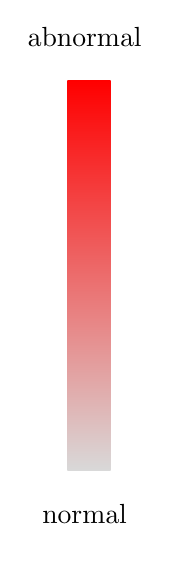
\begin{tikzpicture}[scale=1.1,auto,swap]
    \shade[top color=red,bottom color=gray!30] (0,1.5) rectangle (0.5,6);
    \node[inner sep=0] (corr_text) at (0.2,6.5) {abnormal};
    \node[inner sep=0] (corr_text) at (0.2,1) {normal};
    \node[inner sep=0] (corr_text) at (0.2,0.5) {};
  \end{tikzpicture}
  \caption{mriLargeGaussUnifDirAD}
\end{figure}



% scale parameter for the font size in the circles
\newcommand*{\scaleLabelImg}{0.7}
\begin{figure}[H]
  \centering
  {\scalefont{\scaleLabelImg}
  \begin{tikzpicture}[scale=1.0,auto,swap]

  % the two brain figures on top
  \node (brain) at (0,1.5) { \includegraphics*[scale=\scaleLabelImg]{\midLateralLoc/Mid-Lateral_surface3.eps}};

  % the 6 circles
  \draw[scale=\scaleLabelImg] (-9,-6) circle [radius=2cm] node {BIOMK1};
  \draw[scale=\scaleLabelImg] (-4,-6) circle [radius=2cm] node {BIOMK2};
  \draw[scale=\scaleLabelImg] (1,-6) circle [radius=2cm] node {BIOMK3};
  \draw[scale=\scaleLabelImg] (-9,-10.5) circle [radius=2cm] node {BIOMK4};
  \draw[scale=\scaleLabelImg] (-4,-10.5) circle [radius=2cm] node {BIOMK5};
  \draw[scale=\scaleLabelImg] (1,-10.5) circle [radius=2cm] node {BIOMK6};

  \end{tikzpicture}
  }

  \caption{Labels of the different areas analysed}
\end{figure}

\end{document}

